\documentclass[a4paper]{article}

\usepackage[english]{babel}
\usepackage[utf8]{inputenc}
\usepackage{graphicx}
\usepackage[top=0.8in, bottom=0.9in, left=1in, right=1in]{geometry}
\usepackage{amsmath}
\usepackage{setspace}
\usepackage{hyperref}
\usepackage{listings}
\usepackage{courier}
\usepackage[export]{adjustbox}
\usepackage[english]{babel}
\usepackage[colorinlistoftodos]{todonotes}
\usepackage[]{algorithm2e}
\makeatletter
\newcommand*{\myfnsymbolsingle}[1]{%
  \ensuremath{%
    \ifcase#1% 0
    \or % 1
    \dagger
    \or % 2
     \dagger 
    \or % 3  
     \dagger
    \or % 4   
      \mathsection
    \or % 5
      \mathparagraph
    \else % >= 6
      \@ctrerr  
    \fi
  }%   
}   
\makeatother

\newcommand*{\myfnsymbol}[1]{%
  \myfnsymbolsingle{\value{#1}}%
}

% remove upper boundary by multiplying the symbols if needed
\usepackage{alphalph}
\newalphalph{\myfnsymbolmult}[mult]{\myfnsymbolsingle}{}

\renewcommand*{\thefootnote}{%
  \myfnsymbolmult{\value{footnote}}%
}



\title{Image Inpainting Using Markov Random Field Filter and Cahn-Hilliard Equation}

\author{Hongzi Mao, Tianyu Wang}
\begin{document}
\maketitle
\begin{abstract}
\noindent
We employed two general methods to recover polluted images. For gray scale images, we used Markov Random Field (MRF) method to fill in the polluted pixel based on exiting neighborhood pixels. In practise, we faciliated multiway swiping and global searching to further improve MRF inpainting result. For binary images, we adopt \emph{Cahn-Hilliard} model to reconstruct the whole image. Some preliminary inpainted result are attached as example.
\end{abstract}

\begin{spacing}{1.4}
\section{Introduction}
There are many cases that images get polluted by variant accidental instances. For example, old photos, sonar pictures and medical images are usually containing unexpected non-negotiable dark points and dark lines. Even modern digital images may contain some accidentally added text or geometry structures. These unwanted parts on image are conspicuous and annoying. Therefore naturally, one may desire a tool to fix these parts by fill in `original' image. However the information of original image on these holes are erased by the pollution. The best we can do is to fit in these missing part based on the given damaged image. Most of times, these bad parts have relatively small size, and the original image contains inside is very likely to look like the undamaged surrounding part. In practice, many photographers use this technique manually on Photoshop to reconstruct these missing parts. In order to achieve this in an efficient way, Markov Field$^{[1]}$ and Cahn-Hilliard Equation$^{[2]}$ are adopted. Markov Field Filter will assign a gray scale intensity to a particular pixel depending only on the intensities of the pixels in a certain neighborhood of that particular pixel. Cahn-Hilliard Equation method will use an approximation to the original image which is uniform on the whole domain and close to the original image outside the inpainted area. One may expect that the Markov Field Filter will not change any part outside the area which is intented to be inpainted, whereas the Cahn-Hilliard Equation method will give a completely new image.\\
\section{Markov Random Field Filter}
\subsection{Models}
For simplicity, we use M$\times$N matrix to model grey scale image. Generally speaking, the probability for picking a particular intensity on a polluted pixel at $(i, j)$ can be expressed as $P(I(i, j) | I(i+1, j), I(i-1, j), I(i, j+1), I(i, j-1))$. Here we preliminarily construct 3 models for this expression.\\
$$P = rand(I(i+1, j), I(i-1, j), I(i, j+1), I(i+1, j-1))$$
$$P = rand(I(i+1, j), I(i-1, j), I(i, j+1), I(i+1, j-1), \sum\limits_{(i^*, j^*)\in \Omega(i, j)} I(i^*, j^*)/4) $$
~\\
where \emph{rand} stands for randomly picking value from these candidates and $\Omega$ means neighbor pixels. Intuitively, these 2 models means polluted pixel should has relatively large probability to share similar intensity with its neighbors. In practice, \emph{rand} can be changed to some other distribution functions which utilize the information from given neighbors intensity. \\
~\\
The third model has similar form as above two models. However, it predict a window of pixel intensity at a time, instead of only one pixel intensity as described above. The general expression will be  $P(\Omega(I(i, j)) | \Omega(I(i+s, j)), \Omega(I(i-s, j)), \Omega(I(i, j+s)), \Omega(I(i, j-s)))$, where $\Omega$ means a square of pixel group and s is window size. \\
~\\ 
In practise, we use two techinques to further improve the result. Firstly, the practical inpainting result depends on the way how inpainting region get swiped. For example, if swiped top down, then the inpainted region will be more similar as the pixels on its top. In order to compensate for this bias, we perform two independent inpainting process, one swipe the image top-down left-right, the other in opposite direction. At the end, these two results are merged together.\\
~\\
Secondly, sometimes some region is highly polluted and the pixel information from its neighbors may not be reliable. Therefore, we extend the inpainting pixels candidate from global matching. Specifically, besides the neighbour pixels, we search the entire image to find other pixel candidates, $(i',j')$, such that $ \sum\limits_{(i^{'*}, j^{'*})\in \Omega(i', j'), (i^{*}, j^{*})\in \Omega(i, j)} (I(i^{'*}, j^{'*})-I(i^*, j^*))^2$ is small.\\
\subsection{Result}
The Markov Random Field Filters are in general capable of dealing with inpainting complicated grey scale images. Since the intensities are determined only by a neighborhood of a given cell, the output image tend to be uniform and smooth. In the following example, we used the second model in the local filter and the extention as an illustration. The neighbour pixels diffuse in the polluted part for local inpainting, while the non-local filter may perform better at some region but might also introduce unexpected edges. 
\begin{center}
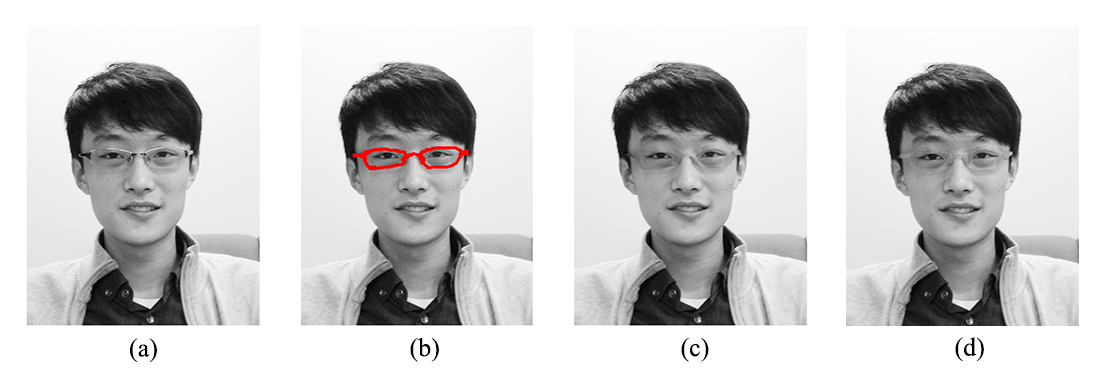
\includegraphics[height=2in]{1.png}\\
\scriptsize
Fig 1. (a). Original gray image. (b). Manually selected mask (c). Local MRF inpainting result (d). Global extension inpainting result.
\end{center}
\normalsize
\section{Cahn-Hiliard Method}
\subsection{Model}
We adopt the energy function from Bertozzi et al.$^{[2]}$, where the modified Cahn-Hilliard equation describes the energy in the whole image domain $\Omega$:\\
$$ E_{1} = \int \limits_\Omega \frac{\epsilon}{2}(\nabla u)^2+\frac{1}{\epsilon}u^2(u-1)^2 dxdy$$ 
For the unpolluted area, the field energy function is:\\
$$ E_{2} = \lambda_{0} \int \limits_{\Omega\slash D} (f-u)^2 dxdy$$
The constrain term $u^2(u-1)^2$ will guide the intensity of pixel to be inpainted tend to have black or white pixel.\\
~\\
The derivation of Euler-Lagrange Equation for first energy equation is as follows:\\
\begin{align}
&\frac{E_1(u+\delta v)- E_1(u)}{\delta} \notag\\
&= \frac{1}{\delta} \int \limits_\Omega \frac{\epsilon}{2}(\nabla u +\delta \nabla v)^2 + \frac{1}{\epsilon}(u+\delta v)^2(u+\delta v-1)^2 - \frac{\epsilon}{2}(\nabla u)^2 - \frac{1}{\epsilon}u^2(u-1)^2 dxdy \notag\\
 &= \frac{1}{\delta} \int \limits_\Omega \frac{\epsilon}{2}(2\delta\nabla u\nabla v+\delta^2 (\nabla v)^2)+\frac{1}{\epsilon}((u^2+2\delta u v+\delta^2 v^2)(u^2+2u(\delta v -1) +\delta^2 v^2-2\delta v +1))dxdy\notag\\
 &=\frac{1}{\delta} \int \limits_\Omega \frac{\epsilon}{2}(2\delta\nabla u\nabla v)+\frac{1}{\epsilon}(4u^3\delta v - 6 \delta u^2 v + 2\delta u v) + o(\delta^2) dxdy\notag\\
 &=\int \limits_\Omega (-\epsilon \nabla^2 u+\frac{1}{\epsilon}(4u^3-6u^2+2u))v +o(\delta)dxdy\notag
\end{align}
Therefore, the corresponding Euler-Lagrange Equation is:\\
$$-\epsilon \nabla^2 u+\frac{1}{\epsilon}(4u^3-6u^2+2u) = 0$$
The derivation of Euler-Lagrange Equation for second energy equation is:\\
\begin{align}
\frac{E_2(u+\delta v)- E_2(u)}{\delta} &= \frac{\lambda_0}{\delta} \int \limits_{\Omega\slash D}\frac{(f-u-\delta v)^2 - (f-u)^2}{\delta}dxdy\notag\\
&=\lambda_0\int \limits_{\Omega\slash D}-2(f-u)v+o(\delta)dxdy\notag
\end{align}
Therefore, the corresponding Euler-Lagrange Equation is:\\
$$-2\lambda_0(f-u) = 0$$
Combine those two Euler-Langrange Equations above and apply gradient descent method:
$$\frac{du}{dt} = \epsilon \nabla^2 u-\frac{1}{\epsilon}(4u^3-6u^2+2u) +2\lambda(x, y)(f-u)$$
where, $\lambda(x, y) = \lambda_0$ if $(x, y) \in D$, otherwise, $0$.\\
~\\
In practice, we used following approximation method as numerical PDE solver:\\
$$ \frac{du}{dt} \simeq \frac{u^{(n+1)}-u^{(n)}}{\Delta t}$$
In order to get good convergence, $\Delta t$ satisfies $\Delta t \leq min(\frac{(\Delta x)^2}{2\epsilon}, O(\epsilon))$.\\
\subsection{Result}
The Cahn-Hiliard Equation gives us a fine way to implement inpainting on binary images. When the inpainting area has a horizontal or vertical edge connected with unpolluted area, the output is perfect. In other cases, the result may be less excellent for inpainting skewed edge due to the discretizition of a digital image. A limitation of this method is that the outcome depends on the manually indicated inpainting area. If the inpainting area is not properly proposed, it will result in some unpleasing changes. 
\\The example presented below applies the method derived above to a simple binary image. The parameters we used to perform the experiment is, $\epsilon = 0.02, \lambda_0 = 1,000,000, \Delta t = 0.0001$, and 1,000 iterations are performed in gradient descent.\\
\begin{center}
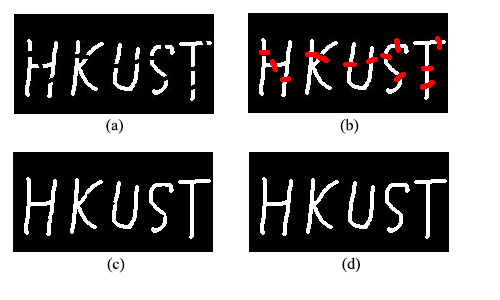
\includegraphics[height=3.5in]{2.png}\\
\scriptsize
Fig 2. (a). Damaged image. (b). Manually selected inpainting region. (c). Inpainted image. (d). Reference image.
\end{center}

\section{Conclusion}\footnote{Source code can be downloaded from: \url{https://github.com/Tony-Mao/image_inpainting}}
Different methods give different results, the Markov Random Field Filter is more capable of dealing with complicated image. Meanwhile, Cahn-Hilliard Equation Method can preserve sharp edges provided that proper parameters are chosen. The Markov Filter Method has been modified in the sense that now the filter will process in two different scanning orders. Each time, in the inpainting region, the filter will progressively recover the pixels starting from different corners, and this in general will give us better results. The Cahn-Hiliard Equation Method produces nice result in the example. But some limitations are encountered in the Cahn-Hiliard Equation Method: firstly the implementation presented in this report is only valid for binary images; secondly, the inpainting region must be manually carefully indicated so that the program can produce a satisfactory result. One may consider using some segmentation technique involving graph cut to automatically extract polluted area as future work. \\
~\\
~\\
~\\
~\\
~\\
~\\
\noindent
\Large
\textbf{References}
\normalsize
\begin{enumerate}
\item Marcelo Bertalmio, Guillermo Sapiro, Vincent Caselles, Coloma Ballester. \textbf{Image Inpainting} \emph{SIGGRAPH} (2000) Proceedings of the 27th annual conference on Computer graphics and interactive techniques p 417-424
\item Andrea Bertozzi, Selim Esedoglu, and Alan Gillette. \textbf{Inpainting of Binary Images Using the Cahn-Hilliard Equation}.\emph{IEEE Transactions in Image Processing}
\item Ryuzo Yokoyama, Robert M. Haralick. \textbf{Texture Pattern Image Generation by Regular Markov Chain}. \emph{Pattern Recognition} Vol.11, pp.225-234
\end{enumerate}

\end{spacing}
\end{document}